\documentclass[a4paper,10pt]{article}
%\usepackage[utf8x]{inputenc}
%\usepackage{wrapfig}
\usepackage{graphicx}    % needed for including graphics e.g. EPS, PS
%\graphicspath{{C:/Users/zilmangroup/Documents/mathematica/images/}} %%%%%%%%%%%%%%%
\graphicspath{{/home/jrothschild/Research/PopDyn_variation/Figures/}} %%%%%%%%%%%%%%%
\usepackage{amsmath, amsthm, amssymb, braket, color} %%%%%%%%%%%%%%%%
\usepackage[usenames,dvipsnames]{xcolor} %%%%%%%%%%%%%
\usepackage{subfig} %For subfigures
\usepackage[normalem]{ulem} %for striking out text
\numberwithin{equation}{section} %%%%%%%%%%%%%%%
\topmargin -1.5cm        % read Lamport p.163
\oddsidemargin -0.04cm   % read Lamport p.163
\evensidemargin -0.04cm  % same as oddsidemargin but for left-hand pages
\textwidth 16.59cm
\textheight 21.94cm
%\pagestyle{empty}       % Uncomment if don't want page numbers
\parskip 0pt           % sets spacing between paragraphs
%\renewcommand{\baselinestretch}{1.5}     % Uncomment for 1.5 spacing between lines
\parindent 8pt          % sets leading space for paragraphs

%opening
\title{Moving the nonlinearity between birth and death.}
\author{MattheW Badali, Jeremy Rothschild}

\begin{document}

\maketitle

%\begin{abstract}
Skip it for now
%\end{abstract}

\section{Introduction} \label{Introduction}% - MattheW
%The application of math to biology has a long history, from Malthus to M\"{u}ller and Pearson, Fisher to Kimura \cite{}. %high-schoolers? Bad intro
Applying mathematics to biology has been a highly successful endeavor, from helping establish historical timescales in phylogenies to describing contemporary distributions of species diversities \cite{Hubbell2001}. %, as well as modelling the dynamics of a population or protein. %citations!
%idk: devo, mutation hypothesis and stats, max entropy in vision, life at low Reynolds number, diffusion in membranes and NMR, phenotypic switches, ESS, predicting vaccines
Deterministic analysis has been a mainstay tool of the mathematical biologist, for instance in modelling the dynamics of competing populations \cite{Chesson1990} or diffusing proteins in a developing organism \cite{Maini2004}. 
Though there has always been a statistical element to the application of math techniques to biology, it is only in recent decades that the application of stochastics has allowed for thorough analysis of probabilistic events, especially rare events that deviate far from the equilibrium of deterministic results. 

With the application of more complex mathematics comes a greater likelihood for error. 
The subdiscipline of bioinformatics suffers from a reputation for drawing conclusions based on correlations \cite{}. %genomics?
More pertinent to this paper, an approximation used both in real-space and momentum-space gives conflicting results \cite{Ovaskainen2010}, despite the approximations seeming mathematically sound in both situations. 
When applying mathematical techniques to biological problems one must take care, and an understanding of how and why a technique works is invaluable in this regard. 
%Even well established tools should not be treated as a black box. 
In this paper we look at how a stochastic problem should be set up, given a deterministic equation as a starting point. 
We will also regard the validity of some approximations commonly applied to stochastic systems. 

The deterministic equation we consider is the logistic equation, one of the most common models to describe a biological system \cite{especially with different q’s}. 
It shows up in epidemiology /cite{Assaf2009,others?}, biodiversity \cite{Hubbell2001?,others?}, and generally as a default for modelling a population that grows to a constant value \cite[bacteria OD, eg]. 
For a population of $n$ individuals, we will be dealing with stochastic equations that give the deterministic limit
\begin{equation}
 \frac{dn}{dt} = r\,n\left(1-\frac{n}{K}\right),
 \label{logistic}
\end{equation}
where $r$ is a rate constant and $K$ is a carrying capacity, a phenomenological measure of the system size. 
The deterministic equation arises as a large population limit of a stochastic system \cite{Nisbet1982/Gardiner2004,others?}; namely it is the difference of the stochastic birth and death rates. 
Thusly, starting from only a deterministic equation there is some freedom to choose the stochastic rates for birth ($b_n$) and death ($d_n$). 
As the choice of birth and death rates contains ambiguity, researchers have leeway in making their decision, resulting in a variety of similar but distinct models \cite{same as first sentence of paragraph? - see Ovaskainen for a couple}. 

The main goal of this paper is to investigate the impact of this choice on one measurable quantity, the mean time to extinction (MTE). 
Calculation of the MTE, $\tau_e$, falls into a general class of problems in the mathematical subdiscipline of first passage processes within stochastic analysis. 
%This is a well-established field and while the mathematical results in this paper are not novel, the biological interpretations are. 
Given enough time in a stochastic system, it is increasingly likely that a series of fluctuations will bring the system to a state from which it cannot escape, called an absorbing state. 
In a population with randomly occurring births and deaths there is always a chance that a series of deaths will bring the population to extinction, after which it cannot recover. 
The MTE is the mean of the probability distribution of exit times of the system; it gives the timescale on which we expect the species to go extinct. 

Generally a community is made up of many species; mathematically the number of species constrains the dimensionality of the problem \cite{Armstrong1980}. %it’s not equal per se
In most cases, only the one dimensional MTE can be solved exactly \cite?{}. 
In more complicated situations an approximation is necessary, and there exist many such techniques \cite{}. 
These techniques tend to rely on a system size expansion and assume that the population is typically large, a reasonable assumption in most biological systems. 
%We will investigate a few common approximations and compare them to the exact results. %this is said 3 paragraphs earlier?

Along with the comparison of common approximations, this paper seeks to explore the parameter space, and biological meaning therein, of stochastic models of the logistic equation. % as they influence the mean time to extinction. 
%Along with…, this paper seeks to explore various stochastic models of the logistic equation, exploring the parameter space and providing a biological interpretation of these parameters.
First we will introduce the model in more detail. 
Then both the steady state population distribution and MTE will be calculated under different biological assumptions. 
Various common approximation techniques will be investigated and compared to the exact results. 
Finally, a discussion of the results will conclude that increasing the birth and death rates commensurately leads to greater population variance and lesser MTEs, and that the choice of model is of critical importance when establishing a system from which to draw conclusions. 
%using a logistic model without justification allows for only the broadest of results to be credible, with most details being vacuous













\section{Model}% - MattheW

The simplest model of an isolated population has linear birth and death terms (that is, the per capita birth and death rates are constant). 
This model is a classic but gives the outcome of population explosion with some probability\cite{Nisbet1982}. %it’s not a time, it’s a fraction of the instances
%, as probably is the case with constant birth/death (immigration/emigration) or any combination of these two. [find examples]
To mathematically curb this infinite growth, and to biologically allow for intraspecies interactions, a non-linear term is required, and a quadratic is the easiest non-linearity to handle. 
The difference between per capita birth and death gives some rate constant $r$, and this rate constant is inhibited by the density of the population, hence a decrease by $n/K$, giving the desired quadratic term. 
This is exactly the logistic equation \ref{logistic}. 

Extinction occurs at $n=0$, an unstable fixed point of the logistic equation, whereas there is a stable fixed point at $n=K$. 
%The logistic equation \ref{logistic} has fixed points at extinction and the carrying capacity, $n=0$ and $n=K$ respectively. 
Common practice in dynamical systems analysis is to rescale variables to remove parameters and simplify the system. 
Since we are dealing with continuous time we can remove the rate constant from our equation; we do so by rescaling the time by $r$. 
Similarly, in the deterministic equation we could rescale $n$ by $K$ and have no remaining parameters.
However, in the stochastic version we cannot apply this latter rescaling, because of the implicit population scale of $\pm1$ organism for each birth/death event. %or “because the integer number of organisms has an implicit population scale of 1.” %organism/individual

Here we have assumed that the stochasticity comes from the discretization of the population, that it must exist at integer values, in opposition with the results of a deterministic model like equation \ref{logistic}. 
Such stochasticity is termed demographic noise. 
Instead of a birth rate $b_n$ we assume that each birth event is independent and distributed exponentially with a probability $b_n\,dt$ of occuring in each infinitesimal time interval $dt$, and this is similarly assumed for death events. %too technical? Or esoteric?
In this paper we use the birth rate
\begin{equation}
 b_n = \Big(1 + \frac{\delta}{2}\Big)\,r\,n - \frac{q\,r}{K}n^2% = r\,n\left(1+\frac{\delta}{2}-q\,n/K\right)
\label{birth}
\end{equation}
and death rate
\begin{equation}
 d_n = \frac{\delta}{2}\,r\,n + \frac{(1-q)r}{K} n^2 = r\,n\left(\frac{\delta}{2}+(1-q)\,n/K\right).
\label{death}
\end{equation}
Note that we introduce two new parameters in our equations \ref{birth} and \ref{death}: $q\in[0,1]$ shifts the nonlinearity between the death term and the birth term whereas the parameter $\delta\in[0,\infty)$ establishes a scale for the contribution of linear terms in both the birth and death rates.
We include the parameter $\delta$ to account for the stochastic relevance of the absolute values of the per capita birth and death rates, but in the deterministic limit only their difference $r$ affects the dynamics of the system. 
Parameter $q$ describes where the intraspecies inhibition acts: a high $q$ near unity implies competition for resources and a decreased effective birth rate, whereas a low $q$ near zero reflects more direct conflict, with intraspecies interactions resulting in greater death rates of organisms. 
%In this formulation we can vary the strength of the density-dependence in the per capita death and birth rates by the factor $q$.
It can be readily checked that $b_n-d_n$ recovers the right-hand side of equation \ref{logistic} where, as per design, the new parameters $q$ and $\delta$ do not appear.
The choice of these parameters specifies a particular model and has consequences on the MTE. 
%We will find that this choice has consequences on the MTE. %and pdf

The model described above has one other notable feature. 
Except at $q=0$, there is a population at which the competition brings the effective birth rate to zero. 
This is the maximum size the population can achieve, and we define this cutoff as
%This limits the population to a maximal size $N = \lceil n_{max}\rceil$, where $n_{max}$ is defined as the population size such that $b_{n_{max}}=0$.
%From equation \ref{birth} we find that
\begin{equation}
N = \frac{K}{q}\Big(\,1 + \frac{\delta}{2}\,\Big).
\label{maxN}
\end{equation}
Therefore we limit our calculations to the biologically relevant range $n\in[0,N]$. % and, for completeness to our study, we can readily check that for our range of parameters $N\geq K$. 
Already it is evident that the ``hidden" parameters of $\delta$ and $q$ have an effect on the system, as different values of the parameters will naturally define a range of states accessible in the model. 
Note that so long as $q\leq 1$ the death rate is positive semi-definite for the domain of interest. % as defined previously does not imply any necessary subtle manipulation of the population range since the death rate is always positive (except at $n=0$) in the range of $q$ and $\delta$ described earlier. 
%The lower bound of the population range for all models is at our unstable fixed point representing an extinct species $n=0$.
At $n=0$ both the birth and death rates go to zero: this is the stochastic absorbing state. 



















\section{Quasi-stationary Probability Distribution Function}% - Jeremy

A probability distribution function is a useful mathematical tool to describe the state of a dynamical system.
We define $P_n(t)$ as the probability that the population is composed of $n$ organisms at time $t$.
The evolution of the distribution in our single birth and death process is captured in the master equation
\begin{equation}
\frac{dP_n}{dt} =  b(n)P_{n-1}(t) + d(n)P_{n+1}(t) - (b(n)+d(n))P_n(t).
\label{master-eqn}
\end{equation}
Note that ultimately at large times the probability of being at population size $n\neq 0$ decays to zero, as more and more of the probability gets drawn to the absorbing state.
%This is due to the stochasticity of the births and deaths and the nature of the absorbing state $n=0$ with no possibility of recovery [reference probability distribution leaking to zero definitely].
%Although this is an important property of this model, it is difficult to describe any dynamics of our model with such a distribution.
Prior to reaching extinction, the system tends toward a quasi-stationary distribution. 

We are interested in this conditional probability distribution function $P_n^c$: the probability distribution of the population conditional to not being in the extinct state: %stationary 
\begin{equation*}
P_n^c = \frac{P_n}{1-P_0}.
\end{equation*}
This dynamics of the distribution are described in a slightly different master equation than equation \ref{master-eqn}:
\begin{equation}
\frac{dP_n^c}{dt} =  b(n-1)P_{n-1}^c(t) + d(n+1)P_{n+1}^c(t) - (b(n) + d(n) - P_1^c(t)d(1))P_n^c(t). 
\label{masters2}
\end{equation}
After an initial transient period, this conditional probability will stabilize to some steady $\tilde{P}^c_n$ for which $d\tilde{P}_n^c/dt=0$. 
The steady state of this distribution is referred to as the quasi-stationary distribution (QSD?), not to be confused with the true stationary distribution of the population which is the state where $\tilde{P}_n(t \leftarrow \infty)=\delta_{n,0}$. 

One way to obtain the quasi-stationary distribution is to exploit equation \ref{masters2} in an algorithm in which we iteratively calculate the change in the distribution $\Delta P^c_n$ in an arbitrarily small time interval $\Delta t$ until all change in the distribution is negligible \cite{Nisbet1982}.
%We start with an arbitrary initial distribution $P^c_n(0)$ and calculate the change $\Delta P^c_n$ for each $n$ in an arbitrarily small time interval $\Delta t$. 
%Thus we obtain a new distribution $P^c_n(\Delta t)$.
%We continue this iterative procedure until the changes in the distribution $|\Delta P^c_n|$ are below a certain threshold.
%Ideally, this iterative process would continue until all $\Delta P^c_n=0$. 
%The accuracy of the algorithm is determined by the time interval $\Delta t$ and reducing this value increases the runtime of the algorithm as more steps are needed to get a steady state solution.
Decreasing the time step $\Delta t$ increases both the accuracy and the runtime, such that an arbitrarily accurate distribution takes a prohibitively long time to calculate. 
We settle for $\Delta P^c_n<\epsilon = 10^{-16}$. %CHECK THIS%Maybe have this in the figure caption - figure goes to probabilities of 10^-20, which is fine, as this -16 is the maximal difference, not necessarily the resolution at the extremes

\begin{figure}[ht!]
  \centering
  \subfloat[\emph{Probability distribution with $\delta=1.00$ and $K=100$}]{\includegraphics[width=0.5\textwidth]{Figure1-A}\label{qsd:q}}
  \hfill
  \subfloat[\emph{Probability distribution with $q=0.06$ and $K=100$}]{\includegraphics[width=0.5\textwidth]{Figure1-B}\label{qsd:delta}}
  \caption{\emph{Probability distribution of the population} The conditional probability distribution functions as found using the quasi-stationary distribution algorithm. Note that for each curve, the population cutoff $N$ is outside the domain presented here. In \ref{qsd:q} increasing lightness indicates an increase in $q$. Similarly, the lightness increase in \ref{qsd:delta} corresponds to an increase in $\delta$}
  \label{qsd}
%The range along the horizontal axis does not fully cover the population, it is truncated to show the relevant region of the distribution. In fact each curve has a different range as the parameters $\delta$ and $q$ vary the maximum population size according to equation \ref{maxN}.
\end{figure}

Results of this algorithm, for different values of $q$ and $\delta$, are presented in Figure \ref{qsd}. 
Increasing the value of $\delta$ shifts the mode toward the anterior of the distribution and spreads the distribution out, increasing the variance. 
Decreasing $q$ has a similar effect. %decreasing q gives broader and anterior
%The maximal value of a distribution shifts as we vary either of these parameters. 








\section{Exact Mean Time to Extinction}% - Jeremy

As described earlier, the system ultimately goes to the absorbing extinct state.
The time in which this happens is a random variable, the mean of which is the mean time to extinction $\tau_e$.
For one-species systems it is well known how to exactly solve the mean time to extinction for a one step birth and death process \cite{Nisbet1982,paper this R,T comes from}. 
The mean time of extinction, for a population of size $n$, is
\begin{equation}
\tau(n) = \frac{1}{d(1)} \sum_{i=1}^n \frac{1}{R(i)} \sum_{j=i}^N T(j)
\label{analytic_mte}
\end{equation}
where
\begin{equation*}
R(n) = \prod_{i=1}^{n-1} \frac{b(i)}{d(i)} \quad \textrm{and} \quad T(n) = \frac{d(1)}{b(n)}R(n+1).
\end{equation*}
Combining equations \ref{birth} and \ref{death} with the solution for the mean time to extinction \ref{analytic_mte} we obtain a complicated analytical expression in the form of a hypergeometric sum.
A typical trajectory starting from $n$ goes first to the deterministic fixed point $K$ and fluctuates about that point before a large fluctuation leads to its extinction. 
%The mean time to extinction depends on the initial population size $n$, however 
Since the time for the population to reach carrying capacity is insignificant compared to the extinction time, the MTE is largely independent of the initial population, and we write $\tau (n) \approx \tau_e$ for all $n$. 
It is well known that $\tau_e$ goes like $e^K$ \cite{Ovaskainen2010} and this is indeed what we observe, see supplemental information. 
What is less well known is the dependence on the hidden parameters, which we detail below. 
\iffalse
%%%%%%%%%%%%APPENDIX%%%%%%%%%%%%%%
\begin{figure}[ht!]
\centering
\includegraphics[width=0.6\textwidth]{MTE_vsK (4 lines at lowlow, highhigh, highlow, lowhigh}
\begin{figure}[ht!]
\centering
\includegraphics[width=0.6\textwidth]{MTE_QvsD_K100_100}
\caption{\emph{Lorum ipsum} So many words..} \label{otherlabel}
\end{figure}
\end{figure}
%%%%%%%%%%%%%%%%%%%%%%
\fi
\begin{figure}[ht!]
\centering
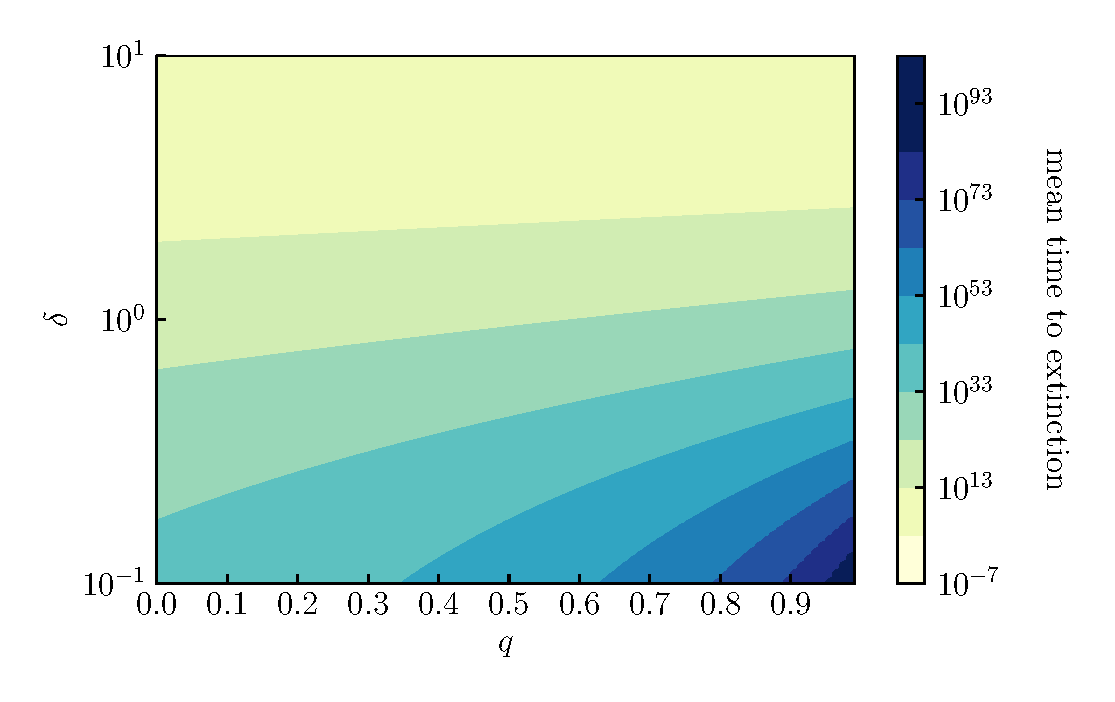
\includegraphics[width=0.6\textwidth]{Figure2}
\caption{\emph{Exploring the mean time to extinction in the parameter space} Recall that $q$ shifts the nonlinearity between the birth and death rates: for $q=0$ the nonlinearity is purely in the death rate, for $q=1$ nonlinearity appears only in birth. The birth and death rates are increased simultaneously with $\delta$.} \label{mteCP}
\end{figure}

The numerical results of this finite sum are summarized in Figure \ref{mteCP}.
It is evident that the MTE depends on the values of $\delta$ and $q$, parameters that appear in the births and deaths but do not appear in the deterministic equation. 
%Increasing $\delta$ causes $\tau$ to decrease whereas increasing $q$ has the effect of increasing $\tau$. 
%We can synonymously describe these phenomena in the language of population dynamics:
Increasing the scaling of the linear terms $\delta$ in birth and death rates has a tendency to decrease $\tau_e$. 
On the other hand, shifting the nonlinearity from the death to the birth rate, in other words increasing $q$, causes an increase in $\tau_e$. 
Note however that the effect of $q$ is magnified for smaller values of $\delta$ and weaker for larger values of $\delta$: see Figure \ref{mte}. 

\begin{figure}[ht!]
  \centering
  \subfloat[\emph{Varying $\delta$}]{\includegraphics[width=0.5\textwidth]{Figure3-A}\label{mte:delta}}
  \hfill
  \subfloat[\emph{Varying $q$} ]{\includegraphics[width=0.5\textwidth]{Figure3-B}\label{mte:q}}
  \caption{\emph{Mean time to extinction for varying $\delta$ and $q$} Each line represents a slice in Figure \ref{mteCP}: Figure \ref{mte:delta} are vertical slices which show how, for different values of $q$, the $\delta$ affects $\tau$. Similarly Figure \ref{mte:q} are horizontal slices which show how, for different values of $\delta$, the $q$ affects $\tau$. As in Figure \ref{qsd}, lightness of the line indicates an increase of \ref{mte:delta} $q$ and \ref{mte:q} $\delta$}
  \label{mte}
\end{figure}














/section{Approximations}% - Both

%[Why we need approximations if we have the exact solution.] - Jeremy
As we have shown, for a one-species model it is possible to write down a closed form solution for the MTE $\tau_e$.
However, finding a general solution for the mean time to extinction given multiple populations is not as trivial. 
Models of stochastic processes away from equilibrium are also difficult to study. 
Many approximations have been developed to accommodate these complications. 
These approximations make the calculations possible or reduce the computing runtime significantly, therefore it is important to know which ones to use and when they are applicable. 
Unfortunately the regime of parameter space in which each approximation is valid is not very well understood. 
We evaluate these approximations and compare them to our exact results, in order to gain insight into their utility. 
%Some insights can be gained from evaluating these approximations in situations that are solvable and thus we will present some of these techniques before discussing our results of the exact solution. % to our stochastic model.
\iffalse
%%%%%%%%%%%%%%%%%%%%%%%%%%%%%%%%%%%%%%%%%%


describe?
Mention here?
eq’ns
paragraph
notes
appendix
1D sum


NO
No








Eigenvalue method


No


No - for now




Same as tau 1 sum?


Tau 1 sum
yes
yes


A




1D analytic
(tau1 gives hypergeometric)
no
no




MattheW try this again


QSD algo -> MTE


yes
yes
1/d1P1
B
Just to find MTE


Small n


yes
yes
Eq’n possibly if it exists
C
MattheW: But how tho
if
FP full


yes
yes


D


yes
FP gaussian


yes
yes
Ref 1/d1P1
And eq’n
D


yes
FP approx pdf -> MTE


Yes for pdf, no for tau
yes


D




FP WKB
no
briefly


E


yes
WKB real


yes
yes
Ref 1/d1P1
And eq’n
E


yes
WKB generating
no
briefly


E




%%%%%%%%%%%%%%%%%%%%%%%%%%%%%%%%%%%%
\fi
%D - MattheW
Starting from the master equation \ref{master-eqn} and expanding the $\pm 1$ terms as $P_{n\pm 1} \approx P_n \pm \partial_n P_n + \partial^2_n P_n$ we arrive at the popular Fokker-Planck (FP) equation:
%. This is known as the Van Kampen expansion \cite{}. - actually the Kramers-Moyal expansion \cite{Gardiner2004 or whomever}
\begin{equation}
\partial_t P_n(t) = - \Big( b_n - d_n \Big) \partial_n P_n(t) + \frac{1}{2 K} \Big( b_n + d_n \Big) \partial_n^2 P_n(t).  \label{FP}
\end{equation}
Instead of a difference differential equation for the probability, equation \ref{FP} is a partial differential equation for the probability density. 
The first term on the right hand side is called the drift term and corresponds to the dynamical equation at the deterministic limit, when fluctuations are neglected. 
The second term is the diffusion term and describes the magnitude of the effect of stochasticity on the system. 
A quasi-steady state can be calculated when the time derivative $\partial_t P_n(t)$ is small. 
To simplify the situation further the birth and death rates can be linearized about the fixed point, which implies a Gaussian solution to the FP equation. 
Equation \ref{FP} can also be solved directly to give a MTE \cite{Gardiner2004}. 

%E - Jeremy
Another method frequently studied is the WKB approximation \cite{}.
The WKB method involves approximating the solution to a differential equation with a large parameter (such as $K$) by assuming an exponential solution (an ansatz) of the form
\begin{equation}
P_n \backsim e^{K\sum_i \frac{1}{K^i}S_i(n)}.
\label{ansatz}
\end{equation}
Starting again from the masters equation \ref{master-eqn}, one can immediately apply the ansatz in the probability distribution and solve the subsequent differential equations to different orders in $1/K$\cite{Assaf2016,etc}.%careful, Assaf2016 is an arXiv paper
To leading order, only $S_0(n)$ is needed. 
This method is commonly referred to as the real-space WKB approximation, wherein we obtain a solution for the quasi-stationary probability distribution.
Another method, known as the momentum-space WKB, is to write an evolution equation of the generating function of $P_n$, the conjugate of the master equation, and then apply the exponential ansatz \cite{Generating function stuff}.

%C - MattheW
Rather than approximating the probability distribution function near the fixed point, a different approximation can be done to estimate the probability distribution function near the absorbing state $n=0$. %this still could be formulated simply as a steady state approximation - see Gardiner p.237
If the bulk of the probability mass is centered on $K$ then the probability of being close to the absorbing state is small (note that this is similar to the quasi-stationary approximation, since the flux out of the system is proportional to the probability of being at a state close to $0$). 
Furthermore, we assume that the probability distribution function grows rapidly, away from the absorbing state, such that $P_{n+1}\gg P_n$, whereas neighbouring birth and death rates are of the same order \cite{smalln}. 
Rewriting the master equation \ref{master-eqn} as $\partial_t P_n = \left(b_{n-1} P_{n-1} - b_n P_n \right) + \left(d_{n+1}P_{n+1} - d_n P_n\right)$ we approximate the left hand side as zero and the right hand side as $\left(-b_n P_n \right) + \left( d_{n+1} P_{n+1}\right)$. 
Rearranging this gives $P_n = \frac{b_{n-1}}{d_n}P_{n-1} = \prod_{i=2}^n \frac{b_{i-1}}{d_i} P_{1}$. %make sure it looks nice, like Gardiner
$P_{1}$ can be found by ensuring the probability is normalized; despite the sum extending beyond the region for which $P_{n+1}\gg P_n$ is valid, the probability distribution generated from this small $n$ approximation is qualitatively reasonable. 

\begin{figure}[ht!]
\centering
\includegraphics[width=0.6\textwidth]{Figure4}
\caption{\emph{Techniques for calculating a probability distribution function} A comparison of the different probability distribution approximations show how the described dynamics at equilibrium may differ for various techniques.} \label{pdf_techn}
\end{figure}


%[PDFs can be approximated, as explained earlier] - Jeremy
As we have described, certain of these approximation methods permit the calculation of a quasi-stationary distribution. 
%Hence, a method that can consistently obtain the correct distribution is a powerful tool.
Figure \ref{pdf_techn} gives us an instance of the quasi-stationary distribution as a function of the parameters $q$, $\delta$ and $K$ for each technique. 
%Note that for the shown range of the parameters the WKB approximation and the quasi-stationary algorithm are not distinguishable by eye, though there are indeed slight differences. 
In general, the ability of the techniques to successfully approximate the quasi-stationary distribution depends heavily on the region of parameter space. 
The WKB method appears to be reasonable everywhere, and the FP approximation is only valid for large $K$ except for low $\delta$ and $q$. %for high K, WKB is always good, FP is good except for low low; for low K, WKB still good, FP bad except for low high; others are bad everywhere
%and small n?
It is also possible to obtain the mean time to extinction from these distributions.
As described earlier, the quasi-stationary probability distribution leaks from $P_n$, a non-extinct population, to $P_0$.
As we are dealing with a single step process, the only transition from which we can reach the absorbing state is through a death at $P_1$: all population extinctions must go through this sole state.
The flux of the probability to the absorbing state is thus given by the expression $d(1)P_1$, hence the approximation \cite{textbooks,WKB paper(Assaf2016?)}
\begin{equation}
\tau_e \approx \frac{1}{d(1)P_1}.
 \label{1overd1P1}
\end{equation}
This same equation can be applied to different methods and algorithms that have produced quasi-stationary distributions. % for which we have an expression for $P_1$.

%A - Jeremy%not just here but elsewhere too, I ask: do we want subtitles/subsections? Ie. inline italic sentence fragments: “Reducing the 1D sum”
By omitting negligeable terms from the full solution to the MTE, equation \ref{analytic_mte}, we can heavily reduce the computational runtime in our calculation.
This becomes important at large population sizes, as the the number of terms in the analytical solution scale with the maximal size of the population.
$\tau_1$, the time it takes for the population to go extinct from a size of one individual, is also the first term in our sum and the dominant term in the solution.
Setting $\tau_e ~ \tau_1$ turns out to be a fine approximation.
However it is only a useful approximation for reducing computation runtime: we learn no more about the dependencies of the MTE on $q$ and $\delta$ than we do for the exact solution. 
%!!!We’re writing tau_e. Also b_n and d_n. Also using \delta instead of \delta/2. Also model vs models - use models in general and model for a parameter choice. Also American modeling or UK modelling. Do we ever say pdf or is it always probability distribution (function)?

%Results of the tau_e approximations presented above - Jeremy
Having calculated the MTE using each approximation, we can now compare the results to the exact solution and verify their accuracy in the parameter space of $\delta$ and $q$.
These results are summarized in Figure \ref{mte_techn}.
As with the probability distribution function, the difference between the solution of the approximations and equation \ref{analytic_mte} is dependent on $q$, $\delta$ and $K$. 
Most of the solutions tend to converge at very low $K$, the divergence of each approximation occurring with increasing $K$. 
From this difference we can evaluate in which regime certain approximations work best.
We find that while no approximation works well for large $\delta$, many of them recover the correct scaling in $K$, albeit off by a factor. %yeah?
For all other parameter regimes, $\tau_1$ and the WKB approximation are both reasonable approximations for the exact results. %!!!CHECK if this is true for small n as well
%, and Fokker-Planck QSD? And small n? And full FP%
%I think we need to be a bit more specific with our assessment of the approximations

\begin{figure}[ht!]
\centering
\includegraphics[width=0.6\textwidth]{Figure5}
\caption{\emph{Techniques for calculating the mean time to extinction} Plotted as a function of the carrying capacity, a comparison of the ratio of the MTE of different techniques to that of the 1D sum reveals the ranges for which they are more accurate for approximating $\tau_{e}$.} \label{mte_techn}
\end{figure}








\section{Discussion}
%QUESTION: what is a “model”, in our language? A set of parameters?
%ANSWER: we have one framework that encapsulates many models

%Jeremy
What is the justification for the use of $q$ and $\delta$ in the birth and death rates? 
These parameters are products of the assumptions we made in constructing the mathematical framework and change the behaviour of our models without affecting the deterministic dynamics.
The parameter $\delta$ gives a scale for our birth and death rates.
This scaling differentiates systems with low birth and death rates from those with high turnover, even when the two models would have the same average dynamics. 
%Whereas the difference between the birth and deaths does not distinguish between two such systems, the size of the birth and death rates is relevant.
%Conditional extinction time: MTE propto exp{(beta-mu) t}
Whereas the deterministic dynamics includes only the difference of birth and death and will not distinguish between populations with high or low turnover, the size of the birth and death rates is still of relevance. 
For example, the probability of extinction of a system with linear birth and death rates starting from population $n_0$ goes as $(b_n/d_n)^{n_0}$ \cite{Nisbet1982}.
In this context, the model with high turnover will differ from one with low turnover as the ratio $b_n/d_n$ will depend on the scale, that is to say, on $\delta$. 

Additionally, $q$ determines where the quadratic dependence lies, whether more in the birth or death rate. 
By having $q$ in the birth, we are assuming that the competition, modelled by the quadratic term, slows down the birth rate, for instance in the form of quorum sensing \cite{Nadell2008}. %also “the genetic regulation of growth rate in response to ...nutrient levels (Vulic and Kolter 2001)”
If it were present in the death the supposition is that the competition instead kills off individuals, for example with illness spreading more rapidly in denser populations \cite{}.
%For many real biological populations, $q$ is between zero and one. %not true
Although we have worked with a $q \in [0,1]$, there is no mathematical reason why $q$ could not take values outside this range. 
Negative values of $q$ would increase both rates, meaning that the density dependence would in fact be beneficial for the birth rates, as in the Allee effect \cite{}, and of further significance for the death rates. 
All $q>1$ has the opposite effect of negatively impacting both rates, signifying that population density would reduce both the birth and death rates. %reduce death, ie. advantages of being in a herd
%This can affect the cutoff, so be careful. 

%[PDF and MTE discussions] - Jeremy
Figure \ref{MTECP} summarizes the numerical results of equation \ref{analytic_mte} into a heat map of the mean time to extinction as a function of the two hidden parameters $q$ and $\delta$.
For the range of $q$ and $\delta$ explored, we find that the MTE changes similarly upon decreasing $q$ and increasing $\delta$, although it depends more sensitively on $\delta$. 
%It is quite clear from the heat map that in our range of parameters $\delta$ has a greater effect on the mean time to extinction, signalling that the linear contribution ha.
It is not trivially apparent from the form of the exact analytical solution that the linear contribution to the rates should be more significant. %, given the summation involved.
%maybe because MTE depends most crucially on P_1, ie inherently on low populations, where the linear term dominates the quadratic term?
%Around the mean of the pdf, the linear and quadratic terms are of similar order ($\delta K$ and $q K$, respectively). 
However, we can get an intuition for why this might be the case. 
At small populations, the linear term is of order $\delta$ (for $\delta \geq 1$) and the quadratic terms is of order $q/K$, hence the linear term dominates the small population end of the distribution. 
It is exactly this portion of the distribution that affects the MTE, as seen in equation \ref{1overd1P1}. 

These qualitative results can be readily intuited by considering the effect each of these parameters has on the distribution, see Figure \ref{DFvsd_K100}.
A broader probability distribution function corresponds to a shorter MTE, as probability more readily leaks from the quasi-steady state solution to extinction.
We find that decreasing $\delta$ sharpens the peak of the distribution and slightly shifts the mode posteriorly. 
As before, the reverse is true for varying $q$: similar tendencies are observed when $q$ is instead decreased.
As the population is allowed more variance about the carrying capacity, states further from the fixed point will be explored more frequently, increasing the probability that the system can stochastically go extinct. 
Varying the parameters has another effect on the probability distribution, as the parameters determine the maximum population size, restricting the possible states to those less than the population cutoff. 
It is readily checked, however, that this change in maximum population size has little to no effect on the MTE, by setting manual cutoffs in our numerical analysis and comparing the results to the true MTE; see supplement. 

%[Approximations] - MattheW
%Fit to e^K? asymptotics? 
%try q=1 for analytic - with d=0 this never dies!!
%recheck analytic forms
%look specifically at these forms at d=q=0, to compare with e^K/K
%maybe compare to asymptotic forms of the sum, like (KK HypergeometricPFQ[{1, 1}, {2, 2 + dd KK}, (1 + dd) KK])/(1 + dd KK)
%or
%(KK HypergeometricPFQ[{1, 1, 1 - KK/qq - (dd KK)/qq}, {2, -(2/(-1 + qq)) - (dd KK)/(-1 + qq) + (2 qq)/(-1 + qq)}, qq/(-1 + qq)])/(1 + dd KK - qq)
Regarding the approximations, the best candidate in most regimes appears to be the WKB approximation. 
It generalizes to multiple dimensions without conceptual difficulty.
Mathematically, at higher dimensions WKB necessitates solving a Hamiltonian system, in order to find a likely route to extinction along which to integrate; an analytic solution cannot be derived in general, and a symplectic integrator is necessary to find the numeric trajectory \cite{}. 
Nevertheless, in our one-dimensional case we find an analytic expression for the mean time to extinction using the WKB approximation.% to be
%\begin{equation}
%\tau_{\text{WKB}} = \frac{1}{\delta+(1-q)/K} \sqrt{2 \pi K} \sqrt{\frac{(1+\delta-q)^2}{\delta q + (1-q)(1+\delta)/K}} \exp \left{ K\left( %\frac{1+\delta}{q}\ln\left[\frac{K(1+\delta)-1}{K(1+\delta-q)}\right] + %\frac{\delta}{1-q}\ln\left[\frac{K\delta+(1-q)}{K(1+\delta-q)}\right] \right) + 
%\ln\left[\frac{K(1+\delta)-q}{K\delta + (1-q)}\right] \right}.
%\end{equation}
We can contrast this with the Gaussian approximation to the Fokker-Planck equation, which always gives an analytic result.%,
%\begin{equation}
%\tau_{\text{FP gaussian}} = \frac{2}{1+2\delta} \sqrt{2 \pi K (1+\delta-q)}
%\exp\left{ \frac{K}{2(1+\delta-q)} \right}.
%\end{equation}
%\begin{equation}
%\tau_{\text{FP WKB}} = \frac{1}{\delta+(1-q)/K} \sqrt{2 \pi K (1+\delta-1)}
% \exp\left{ K\frac{2(1+\delta-q)}{(1-2q)^2} \ln\left[ \frac{K 2(1+\delta-q)}{K(1+2\delta)+(1-2q)} %\right] - \frac{K-1}{(1-2q)} \right}
%\end{equation}
Both formulae are dominated by their exponential dependence on $K$. 
This is to be expected, as the true solution with $\delta,q = 0$ increases as $\frac{1}{K}e^K$ \cite{Lande1993}. 
%WE SHOULD CHECK THIS FOR JUST DELTA OR JUST q=0, TO SEE IF THERE IS A NICE FORM OF THE SOLUTION IN THESE LIMITS, TO WHICH WE CAN COMPARE - there isn’t, it’s all hypergeometric
It is the prefactor multiplying with the carrying capacity in the exponential that is of critical importance in determining the qualitative behaviour of the MTE. 
Lacking an analytical form for this prefactor in the exact solution, we can compare these prefactors in each approximation. 
The Gaussian Fokker-Planck solution has a prefactor $\frac{1}{2(1+\delta-q)}$, so we expect it to underestimate $\tau_e$ in the low parameter regime. %hopefully this is shown in the figure
%The WKB approximation has prefactor $\frac{1+\delta}{q}\ln(1+\delta) + \frac{\delta}{1-q}\ln(\delta) - \frac{1+\delta-1}{q(1-q)}\ln(1+\delta-q)$ for large $K$, which diverges for extremes of $q$ but should otherwise be reasonable. 
To lowest order in $\delta$ and $q$ the WKB approximation has a prefactor of $1-1/K$, which nicely matches the expected limit of 1. 
The WKB approximation matches well for all $\delta$ and $q$ values, as seen in Figures \ref{pdf_techn} and \ref{mte_techn}. 
The other technique that successfully approximates the true probability distribution and mean extinction time is the small $n$ approximation. %!!!CHECK THIS%
It assumes the probability distribution grows rapidly, which is justified for small $n$ and large $K$. 
Since the mean extinction time depends only on $P_1$ this technique gives a reasonable approximation for $\tau_e$. 
%For most of these approximations the behaviour of the mte is in agreement with the exact solution as K grows, however it is off by a factor.
%without an exact solution all we can do is compare these prefactors for each approximation.
%We can find FP QSD prefactor and compare how it ranges with WKB (as that’s a good one.

%MattheW to end - swap these last two paragraphs?

%%%How can experimentalists test this?
How can the MTE be probed in a lab setting? 
%What does this look like in the lab? %what is THIS?
For experimentalists the difficulty of measuring a birth or death rate alone, as it changes with something like population density, varies with the system of interest. 
However, as previously discussed, measuring the average dynamics alone is insufficient. 
%%%With a 96-well plate you can check the pdf
It is possible experimentally to corroborate some of the claims made in this paper. 
For a bacterial species the birth rate could be inferred by the amount of reproductive byproduct present in a sample, for instance factors involved in DNA replication or cell division. %any citations?
The death rate is easily inferred from the birth rate and the average dynamics, or it can be measured using radioisotopes \cite{Servais1985}. %may be more difficult. Maybe with some microfluidics and single cell tracking? 
With these two rates and a couple of 96 well plates it should be a routine procedure to probe the quasi-steady state population probability distribution. 
%%%If you’re patient you could check the tau
A patient experimentalist could also verify the dependence of the MTE on $\delta$ and $q$.  %and low carrying capacity
%!!! CALCULATE HOW LONG THE LENSKI EXPERIMENT SHOULD GO ON FOR%

%%%Consequences of our results
The use of approximations is widespread and necessary when using mathematics to model real systems. 
The takeaway message of this paper is that one must be mindful in their modelling. 
We find that FP, WKB, and small $n$ are largely suitable in the models considered here, in that they recover the correct exponential scaling of the MTE with carrying capacity. 
The biggest caveat is that FP fails for low values of $\delta$ and $q$, and at low $K$.  
Other techniques do not fare so well. 
It is common knowledge that various approximations have situations in which they are more or less applicable. 
%Paragraph?
Mindfulness in modelling not only refers to the method of solution, but to the choice of model itself. 
%%%How other people should use our results
Historically the choice of model seemed to be one of taste or mathematical convenience \cite{again the ones with different q’s}. 
So long as the correct deterministic results were given, the choice of model was not discussed. 
%We have shown that model selection has significant qualitative and quantitative effects on at least two metrics of interest in mathematical biology, including the MTE. 
We have shown that stochastic assumptions have significant qualitative and quantitative effects on at least two metrics of interest in mathematical biology, including the MTE.
%Therefore, we must be diligent in selecting these underlying stochastic dynamics to properly explain the deterministic results of biological phenomena.
%%%The results of others imply certain premises, which could be fine, or could not be fine
This does not invalidate the results of past research, but it does imply that the results are valid only for the hidden parameters chosen at that time, and anyone looking to extend or generalize the results should be wary. %re-reference/cite cases with q=0,1/2
%%%What this means going forward
%all models are valid apriori, all are equally valid in general, but for a particular biological situation we should restrict ourselves to models in a parameter regime defined by the biology
Going forward armed with the knowledge that not all stochastic models are created equal, we argue that one should give careful regard to the biology of relevance when selecting a model. 
Our decisions must be informed by the real world if we are to make models that properly capture this biology. 
%This may seem like a truism but it was not always followed; we hope that our evidence contributes to better practice in the future. 
%%%You’re all wrong and we told you so.

%We have shown that stochastic assumptions have significant qualitative and quantitative effects on at least two metrics of interest in mathematical biology, including the MTE.
%Therefore, we must be diligent in selecting these underlying stochastic dynamics to properly explain the deterministic results of biological phenomena.


\section{References}

\bibliographystyle{unsrt}
\bibliography{collection_18_05_2018}
\bibliography{collection_18_05_2018}

\section{notes to selves}
Need to reference/cite: Allen
MattheW - find small n reference!
Pick and stick with one textbook (Nisbet vs Gardiner)
Have subheadings in italics for the different techniques, whatever?

















































\newpage

\section{PREVIOUSLY: Stochastics}
Consider the stochastic system with birth
\begin{equation}
 b(n) = r\,n - q\,r\,n^2/K = r\,n\left(1-q\,n/K\right)
\end{equation}
and death
\begin{equation}
 d(n) = (1-q)r\,n^2/K.
\end{equation}
When $q=0$ I have the system I've already done some research on.  
In general, $q\in[0,1)$ is a parameter that shifts the nonlinearity between the death term and the birth term.  
Note that, in order to interpret there quantities as rates per infinitesimal time of Poisson processes, or alternately to interpret these are probabilities, both of which are standard characterizations, the quantities must remain positive.  
This leads to some funny business where your birth rate has to be piecewise or else $K/q$ has to be chosen such that it is an integer, leading to a finite domain of integers between $0$ and $K/q$ inclusively ($n\in[0,K/q]|n\in\mathbb{Z}$).  

Solving the backward equation can be done iteratively to get
\begin{equation} \label{etime-approx0}
 \tau_e[n_0] = \sum_{i=1}^{\infty}q_i + \sum_{j=1}^{n_0-1} S_j\sum_{i=j+1}^{\infty}q_i,
\end{equation}
where
\begin{equation}
 q_i = \frac{b(i-1)\cdots b(1)}{d(i)d(i-1)\cdots d(1)}
\end{equation}
and
\begin{equation}
 S_i = \frac{d(i)\cdots d(1)}{b(i)\cdots b(1)}.  
\end{equation}
Again, note that these sums should not go to infinity if the state space is constrained to be finite.  
This can be done, which results in some hypergeometricPFQ functions (according to Mathematica).  
Figure \ref{tauvK} shows the results.  

\begin{figure}[ht]
\centering
\includegraphics[width=0.8\textwidth]{Figure5}
\caption{\emph{Mean time to extinction with the nonlinearity shared between the death and birth rates.}  The red line shows the result when the nonlinearity is purely in the death term.  The blue lines show the shared nonlinearity, with $q$ going from $0.1$ to $0.9$ giving increasing extinction times.  The green lines correspond to a similar model done by Assaf and Meerson (2009) that I have not yet recovered the citation for.  The cyan line is the Moran result (linear in $K$), for reference.  } \label{tauvK}
\end{figure}

Assaf and Meerson (2009) apparently did something similar, though I cannot find that paper at the moment.  
All I have is my interpretation of their results.  
Apparently they have a birth rate something like $b(n)=r\,A\,n + r\,B\,n^2/K$ and a death rate like $d(n)=r\,C\,n + r\,D\,n^2/K$ such that it recovers the appropriate deterministic DE.  

These results shown in figure \ref{tauvK} should be a little disconcerting.  
They suggest that similar models, ones that give the same deterministic equation, can give very different extinction times.  
They are not qualitatively different, in that they are all dominated by their exponential term.  
However, the prefactor of the exponential depends on $q$, and since the scales in biology are typically large ($K\gg1$) this corresponds to drastically different expected mean extinction times.  


\section{WKB}
to come:  you can do a similar breakdown using the WKB method of Meerson et al, and come to similar results



\end{document}


